\section{Testing}\label{sec:test}

  \subsection{Unit Tests}\label{sec:test-unit}

    Adding support to build and run unit tests can be done using the commands given here
    in Listing~\ref{lst:test-unit}.

    \begin{lstlisting}[language=bash,
                       caption={Compiling and Running Unit Tests},
                       label={lst:test-unit}]
      ./autogen.sh --enable-tests
      make check
      make -j8
    \end{lstlisting}

    If everything completes successfully a test suite summary should be given similar to
    what is given here in Listing~\ref{lst:test-unit-summary}.

    \begin{lstlisting}[caption={Test Suite Summary},
                       label={lst:test-unit-summary}]
      PASS: test-dcs-core
      ============================================================================
      Testsuite summary for dcs 0.2.0
      ============================================================================
      # TOTAL: 1
      # PASS:  1
      # SKIP:  0
      # XFAIL: 0
      # FAIL:  0
      # XPASS: 0
      # ERROR: 0
      ============================================================================
    \end{lstlisting}

  \subsection{Coverage Reports}\label{sec:test-cov}

    \begin{lstlisting}[language=bash,
                       caption={Generating Coverage Reports},
                       label={lst:test-cov}]
      ./autogen.sh --enable-coverage --enable-tests
      make -j8
      make check
      make coverage
    \end{lstlisting}

    \begin{lstlisting}[caption={Coverage Summary},
                       label={lst:test-cov-summary}]
      %Writing data to ../lcov.info
      %Summary coverage rate:
        %lines......: 55.6% (1167 of 2100 lines)
        %functions..: no data found
        %branches...: no data found
      %/usr/bin/mkdir -p ../tests/coverage
      %git_commit=`GIT_DIR=../.git git log -1 --pretty=format:%h 2>/dev/null`;\
      %genhtml --title "dcs 0.2.0 $git_commit" \
        %--output-directory ../tests/coverage ../lcov.info
      %Reading data file ../lcov.info
      %Found 50 entries.
      %Found common filename prefix "/home/gjohn/Dropbox/Projects/opendcs/dcs"
      %Writing .css and .png files.
      %Generating output.
      %Processing file src/libdcs-core/dcs-meta-factory.vala
      %... a bunch more lines like the last ...
      %Writing directory view page.
      %Overall coverage rate:
        %lines......: 55.6% (1167 of 2100 lines)
        %functions..: no data found

      %lcov report can be found in:
      %file:///home/gjohn/Dropbox/Projects/opendcs/dcs/tests/coverage/index.html

      %make[1]: Leaving directory '/home/gjohn/Dropbox/Projects/opendcs/dcs/tests'
    \end{lstlisting}

  \subsection{REST APIs}\label{sec:test-rest}

    Testing of the REST APIs outlined in Section~\ref{sec:rest} was performed
    using the Postman application as a client, which allows the automation of
    testing routes by running collections of HTTP requests of any type. For our
    purposes the only types tested needed to be PUT, GET, POST, and DELETE,
    these being sufficient to validate the CRUD model of the objects. The
     relationship between HTTP requests and a CRUD model are PUT to Create, GET
    to Read, POST to Update, and DELETE to Delete.

    Postman allows for test suites to be defined as part of a collection, along
    with each request the data response can be interrogated to determine if the
    contents were what was requested. Figure~\ref{fig:test-postman-def} shows
    the application running with an example of one such test.

    \begin{figure}[H]
      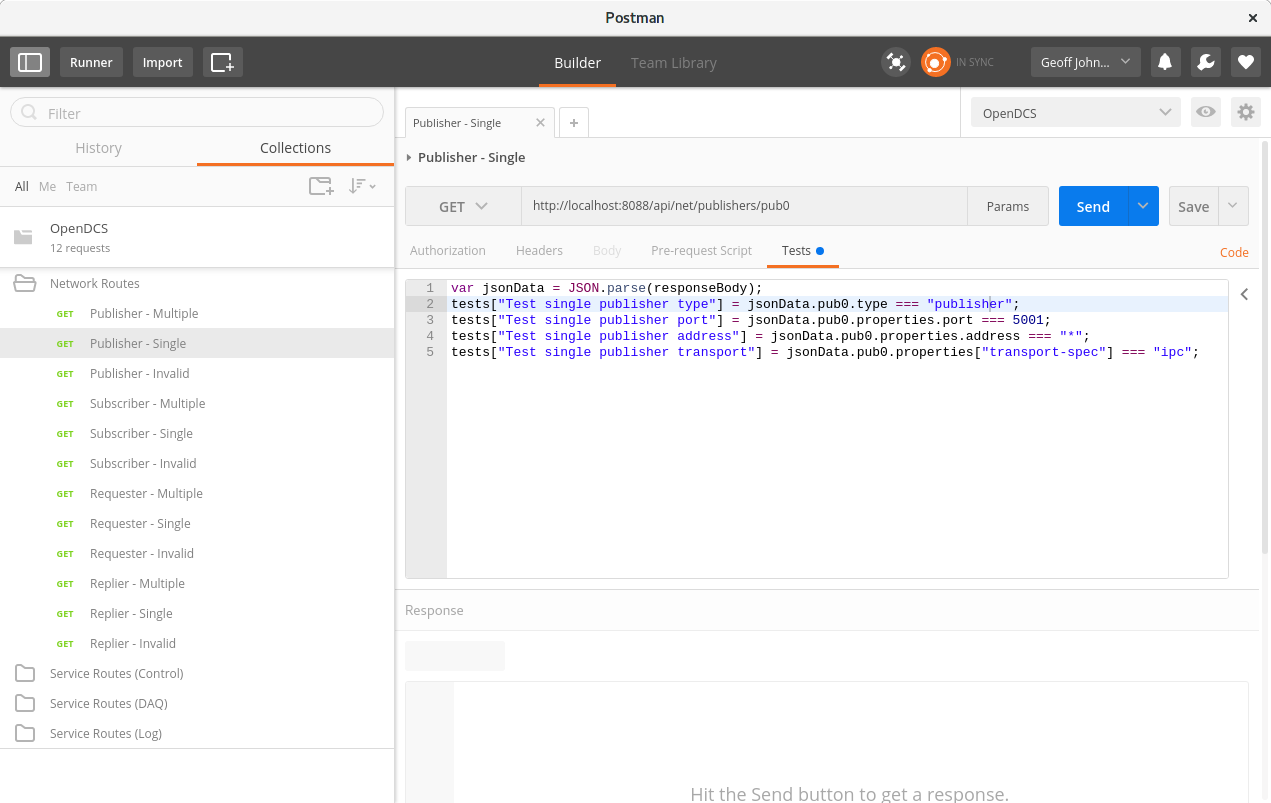
\includegraphics[width=\textwidth]{figures/testing/postman-test-definition}
      \caption{Example of a Test Definition in Postman}
      \label{fig:test-postman-def}
    \end{figure}

    Once the collection of requests and tests have been defined the runner
    allows you execute all at once, or by selecting a sub scope if child
    folders within the collection have been used. An example of a completed set
    of tests is given below in Figure~\ref{fig:test-postman-runner}.

    \begin{figure}[H]
      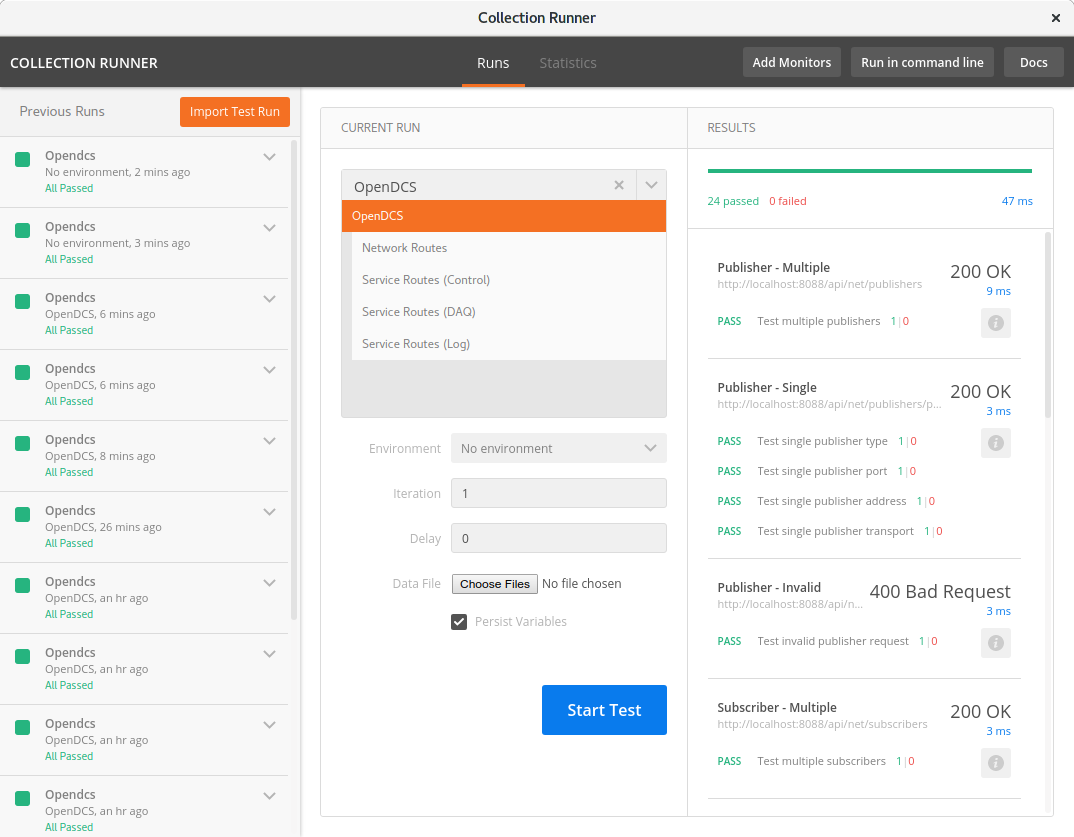
\includegraphics[width=\textwidth]{figures/testing/postman-sample-run}
      \caption{Example Output from Postman Collection Runner}
      \label{fig:test-postman-runner}
    \end{figure}

    Showing the complete set of tests that have been defined in the collection,
    as well as a complete run of tests would be difficult to display in this
    document so an exported copy of the collection will be included on a disc
    along with this report. The complete test results will be given for each of
    the sections on the specific context being tested.

    As mentioned the Postman application affords the ability to run HTTP
    requests as well as define a message body for types that can have one, and
    Javascript test sections that can determine if the content of the result
    was what was expected. The examples below show the test definitions that
    were used to test all CRUD elements of the system. The DcsNetPublisher
    object is used as the type, but all others are identical other than the
    type. The configuration file that was loaded into the service under test is
    given in Section~\ref{sec:test-rest-net}, Listing~\ref{lst:test-rest-net}.

    \subsubsection{Example GET Test for a Request of Multiple Objects}\label{sec:test-rest-get-mult}

      Request string: \texttt{http://localhost:8080/api/net/publishers}

      \begin{lstlisting}[language=Javascript,title=GET Multiple Objects Tests,nolol]
        var jsonData = JSON.parse(responseBody);
        tests["Test multiple publishers"] = jsonData.publishers.length === 2;
      \end{lstlisting}

      \begin{lstlisting}[language=Javascript,title=GET Multiple Objects Response,nolol]
        {
          "publishers": [
            {
              "pub0": {
                "type": "publisher",
                "properties": {
                  "port": 5001,
                  "address": "*",
                  "transport-spec": "ipc"
                }
              }
            },
            {
              "pub1": {
                "type": "publisher",
                "properties": {
                  "port": 5002,
                  "address": "127.0.0.1",
                  "transport-spec": "tcp"
                }
              }
            }
          ]
        }
      \end{lstlisting}

    \subsubsection{Example GET Test for a Request of a Single Object}\label{sec:test-rest-get}

      Request string: \texttt{http://localhost:8080/api/net/publishers/pub0}

      \begin{lstlisting}[language=Javascript,title=GET Single Object Tests,nolol]
        var jsonData = JSON.parse(responseBody);
        tests["Test single publisher type"] = jsonData.pub0.type === "publisher";
        tests["Test single publisher port"] = jsonData.pub0.properties.port === 5001;
        tests["Test single publisher address"] = jsonData.pub0.properties.address === "*";
        tests["Test single publisher transport"] = jsonData.pub0.properties["transport-spec"] === "ipc";
      \end{lstlisting}

      \begin{lstlisting}[language=Javascript,title=GET Single Object Response,nolol]
        {
          "pub0": {
            "type": "publisher",
            "properties": {
              "port": 5001,
              "address": "*",
              "transport-spec": "ipc"
            }
          }
        }
      \end{lstlisting}

    \subsubsection{Example GET Test for a Request of an Invalid Object}\label{sec:test-rest-get-null}

      Request string: \texttt{http://localhost:8080/api/net/publishers/pub2}

      \begin{lstlisting}[language=Javascript,title=GET Single Invalid Object Tests,nolol]
        var jsonData = JSON.parse(responseBody);
        tests["Test invalid publisher request"] = jsonData.publishers.status === 501;
      \end{lstlisting}

      \begin{lstlisting}[language=Javascript,title=GET Single Invalid Object Response,nolol]
        {
          "publishers": {
            "status": 501,
            "error": "Object not found"
          }
        }
      \end{lstlisting}

    \subsubsection{Example PUT Test for a Request of an Object}\label{sec:test-rest-put}

      Request string: \texttt{http://localhost:8080/api/net/publishers/pub2}

      \begin{lstlisting}[language=Javascript,title=PUT Object Request Body,nolol]
        {
          "pub2": {
                "type": "publisher",
                "properties": {
                  "port": 5010,
                  "address": "*",
                  "transport-spec": "tcp"
                }
            }
        }
      \end{lstlisting}

      \begin{lstlisting}[language=Javascript,title=PUT Object Tests,nolol]
        var jsonData = JSON.parse(responseBody);
        tests["Test create publisher request"] = jsonData.publishers["PUT"] === "complete";
      \end{lstlisting}

      \begin{lstlisting}[language=Javascript,title=PUT Object Response,nolol]
        {
          "publishers": {
            "PUT": "complete"
          }
        }
      \end{lstlisting}

    \subsubsection{Example POST Test for a Request of an Object}\label{sec:test-rest-post}

      Request string: \texttt{http://localhost:8080/api/net/publishers/pub2}

      \begin{lstlisting}[language=Javascript,title=POST Object Request Body,nolol]
        {
          "pub2": {
                "properties": {
                  "port": 5020,
                  "address": "*",
                  "transport-spec": "tcp"
                }
            }
        }
      \end{lstlisting}

      \begin{lstlisting}[language=Javascript,title=POST Object Tests,nolol]
        var jsonData = JSON.parse(responseBody);
        tests["Test create publisher request"] = jsonData.publishers["POST"] === "complete";
      \end{lstlisting}

      \begin{lstlisting}[language=Javascript,title=POST Object Response,nolol]
        {
          "publishers": {
            "POST": "complete"
          }
        }
      \end{lstlisting}

    \subsubsection{Example DELETE Test for a Request of an Object}\label{sec:test-rest-delete}

      Request string: \texttt{http://localhost:8080/api/net/publishers/pub2}

      \begin{lstlisting}[language=Javascript,title=DELETE Object Request Body,nolol]
        {
          "pub2": {}
        }
      \end{lstlisting}

      \begin{lstlisting}[language=Javascript,title=DELETE Object Tests,nolol]
        var jsonData = JSON.parse(responseBody);
        tests["Test create publisher request"] = jsonData.publishers["DELETE"] === "complete";
      \end{lstlisting}

      \begin{lstlisting}[language=Javascript,title=DELETE Object Response,nolol]
        {
          "publishers": {
            "DELETE": "complete"
          }
        }
      \end{lstlisting}

    \subsubsection{Common Network Routes}\label{sec:test-rest-net}

      The API defined in Section~\ref{sec:rest-common} were those being tested
      in this context, and the configuration used to test against is below in
      Listing~\ref{lst:test-rest-net}.

      \lstinputlisting[language=Javascript,
                       caption={Configuration of Common Network Objects},
                       label={lst:test-rest-net}]
                      {testing/net-config.json}

      When the service is executed with this configuration the command
      \texttt{ss -antp4 | grep dcs-daq} shows the that the HTTP service as well
      as the ZeroMQ sockets have been correctly brought up and have a status of
      \texttt{LISTEN}, and the connecting pairs show \texttt{ESTAB}, this
      output is given in Listing~\ref{lst:test-rest-net-ss}.

      \begin{lstlisting}[caption={Socket Status During Network Test},
                         label={lst:test-rest-net-ss}]
        LISTEN 0 100 127.0.0.1:5002  *:*             users:(("dcs-daq",pid=1410,fd=23))
        LISTEN 0 100 *:5003          *:*             users:(("dcs-daq",pid=1410,fd=56))
        LISTEN 0 100 127.0.0.1:5004  *:*             users:(("dcs-daq",pid=1410,fd=63))
        LISTEN 0 10  *:8080          *:*             users:(("dcs-daq",pid=1410,fd=4))
        ESTAB  0 0   127.0.0.1:5003  127.0.0.1:43256 users:(("dcs-daq",pid=1410,fd=65))
        ESTAB  0 0   127.0.0.1:57294 127.0.0.1:5002  users:(("dcs-daq",pid=1410,fd=36))
        ESTAB  0 0   127.0.0.1:5004  127.0.0.1:34370 users:(("dcs-daq",pid=1410,fd=67))
        ESTAB  0 0   127.0.0.1:5002  127.0.0.1:57294 users:(("dcs-daq",pid=1410,fd=37))
        ESTAB  0 0   127.0.0.1:43256 127.0.0.1:5003  users:(("dcs-daq",pid=1410,fd=64))
        ESTAB  0 0   127.0.0.1:34370 127.0.0.1:5004  users:(("dcs-daq",pid=1410,fd=66))
      \end{lstlisting}

      \paragraph{Test Suite Run for this Scope}\mbox{}\\

      \begin{table}[H]
        \centering
        \begin{tabular}{p{3in} p{3in}}
          \toprule
          \emph{Request} & \emph{Description} \\ [0.5ex]
          \midrule
             GET /api/net/publishers       & Read multiple publishers \\
             GET /api/net/publishers/pub2  &   Read single publisher \\
             GET /api/net/publishers/pub2  &  Read invalid publisher \\
             PUT /api/net/publishers/pub2  &      Create a publisher \\
            POST /api/net/publishers/pub2  &      Update a publisher \\
          DELETE /api/net/publishers/pub2  &      Delete a publisher \\
             GET /api/net/subscribers      & Read multiple subscribers \\
             GET /api/net/subscribers/sub2 &   Read single subscriber \\
             GET /api/net/subscribers/sub2 &  Read invalid subscriber \\
             PUT /api/net/subscribers/sub2 &      Create a subscriber \\
            POST /api/net/subscribers/sub2 &      Update a subscriber \\
          DELETE /api/net/subscribers/sub2 &      Delete a subscriber \\
             GET /api/net/requesters       & Read multiple requesters \\
             GET /api/net/requesters/req2  &   Read single requester \\
             GET /api/net/requesters/req2  &  Read invalid requester \\
             PUT /api/net/requesters/req2  &      Create a requester \\
            POST /api/net/requesters/req2  &      Update a requester \\
          DELETE /api/net/requesters/req2  &      Delete a requester \\
             GET /api/net/repliers         & Read multiple repliers \\
             GET /api/net/repliers/rep2    &   Read single replier \\
             GET /api/net/repliers/rep2    &  Read invalid replier \\
             PUT /api/net/repliers/rep2    &      Create a replier \\
            POST /api/net/repliers/rep2    &      Update a replier \\
          DELETE /api/net/repliers/rep2    &      Delete a replier \\
          \bottomrule
        \end{tabular}
        \caption{REST API Test Suite for Common Network Components}\label{tab:test-rest-net-suite}
      \end{table}

      \newpage
      \paragraph{Test Suite Results}\mbox{}\\

        All tests defined for the suite of network objects completed
        successfully, the results of the tests can be seen in
        Figure~\ref{fig:test-postman-net-suite}.

        \begin{figure}[H]
          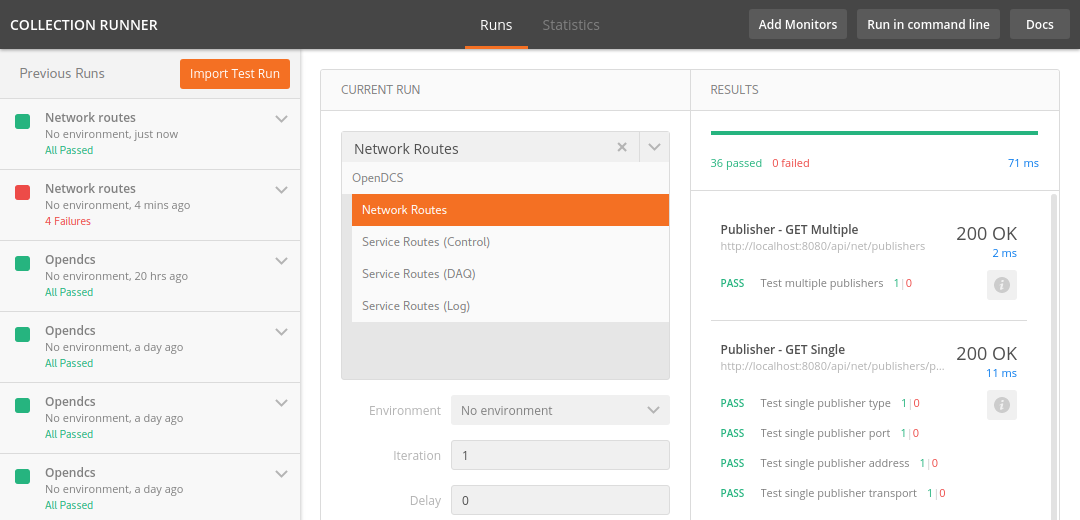
\includegraphics[width=\textwidth]{figures/testing/postman-net-suite-results}
          \caption{Test Suite Results for the Net Objects Tests}
          \label{fig:test-postman-net-suite}
        \end{figure}

    \subsubsection{Data Acquisition Service Routes}\label{sec:test-rest-daq}

      The API defined in Section~\ref{sec:rest-log} were those being tested in
      this context, and the configuration used to test against is below in
      Listing~\ref{lst:test-rest-daq}.

      \lstinputlisting[language=Javascript,
                       caption={Configuration of DAQ Objects},
                       label={lst:test-rest-daq}]
                      {testing/dcs-daq.json}

      When the service is executed with this configuration the command
      \texttt{ss -antp4 | grep dcs-daq} shows the that the HTTP service as well
      as the ZeroMQ sockets have been correctly brought up and have a status of
      \texttt{LISTEN}, and the connecting pairs show \texttt{ESTAB}, this
      output is given in Listing~\ref{lst:test-rest-daq-ss}.

      \begin{lstlisting}[caption={Socket Status During DAQ Tests},
                         label={lst:test-rest-daq-ss}]
        LISTEN 0 100 *:5001          *:*             users:(("dcs-daq",pid=2740,fd=16))
        LISTEN 0 10  *:8080          *:*             users:(("dcs-daq",pid=2740,fd=4))
        ESTAB  0 0   127.0.0.1:53388 127.0.0.1:6001  users:(("dcs-daq",pid=2740,fd=23))
        ESTAB  0 0   127.0.0.1:5001  127.0.0.1:43446 users:(("dcs-daq",pid=2740,fd=24))
        ESTAB  0 0   127.0.0.1:5001  127.0.0.1:43448 users:(("dcs-daq",pid=2740,fd=25))
      \end{lstlisting}

      \paragraph{Test Suite Run for this Scope}\mbox{}\\

      \begin{table}[H]
        \centering
        \begin{tabular}{p{3in} p{3in}}
          \toprule
          \emph{Request} & \emph{Description} \\ [0.5ex]
          \midrule
             GET /api/daq/devices       & Read multiple devices \\
             GET /api/daq/devices/dev1  &   Read single device \\
             PUT /api/daq/devices/dev1  &      Create a device \\
            POST /api/daq/devices/dev1  &      Update a device \\
          DELETE /api/daq/devices/dev1  &      Delete a device \\
             GET /api/daq/sensors       & Read multiple sensors \\
             GET /api/daq/sensors/sen1  &   Read single sensor \\
             PUT /api/daq/sensors/sen1  &      Create a sensor \\
            POST /api/daq/sensors/sen1  &      Update a sensor \\
          DELETE /api/daq/sensors/sen1  &      Delete a sensor \\
             GET /api/daq/signals       & Read multiple signals \\
             GET /api/daq/signals/sig1  &   Read single signal \\
             PUT /api/daq/signals/sig1  &      Create a signal \\
            POST /api/daq/signals/sig1  &      Update a signal \\
          DELETE /api/daq/signals/sig1  &      Delete a signal \\
             GET /api/daq/ports        & Read multiple ports \\
             GET /api/daq/ports/port1  &   Read single port \\
             PUT /api/daq/ports/port1  &      Create a port \\
            POST /api/daq/ports/port1  &      Update a port \\
          DELETE /api/daq/ports/port1  &      Delete a port \\
             GET /api/daq/tasks        & Read multiple tasks \\
             GET /api/daq/tasks/task1  &   Read single task \\
             PUT /api/daq/tasks/task1  &      Create a task \\
            POST /api/daq/tasks/task1  &      Update a task \\
          DELETE /api/daq/tasks/task1  &      Delete a task \\
          \bottomrule
        \end{tabular}
        \caption{REST API Test Suite for DAQ Components}\label{tab:test-rest-daq-suite}
      \end{table}

      \paragraph{Test Suite Results}\mbox{}\\

        All tests defined for the suite of DAQ objects completed
        successfully, the results of the tests can be seen in
        Figure~\ref{fig:test-postman-daq-suite}.

        \begin{figure}[H]
          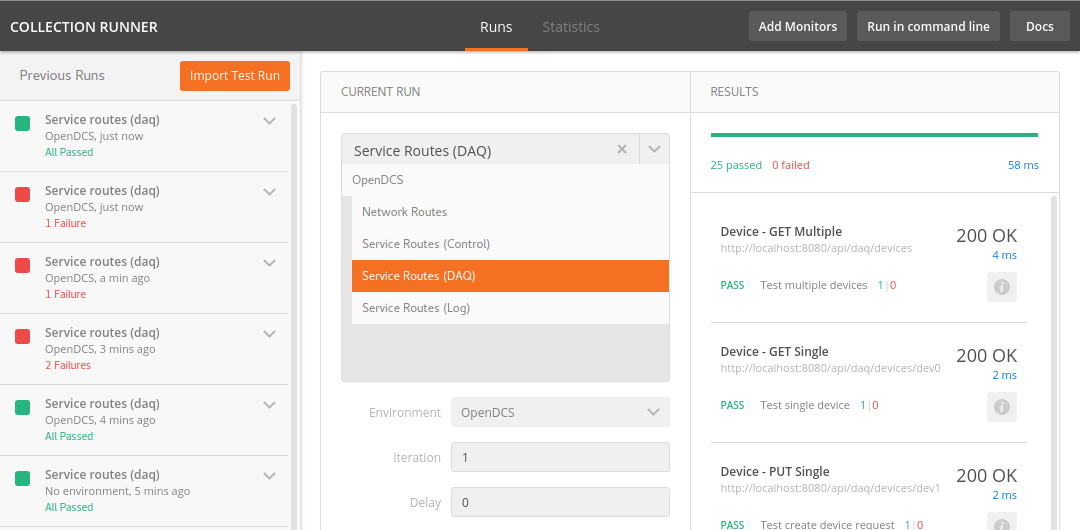
\includegraphics[width=\textwidth]{figures/testing/postman-daq-suite-results}
          \caption{Test Suite Results for the DAQ Objects Tests}
          \label{fig:test-postman-daq-suite}
        \end{figure}

    \subsubsection{Data Logging Service Routes}\label{sec:test-rest-log}

      The API defined in Section~\ref{sec:rest-log} were those being tested in
      this context, and the configuration used to test against is below in
      Listing~\ref{lst:test-rest-log}.

      \lstinputlisting[language=Javascript,
                       caption={Configuration of Log Objects},
                       label={lst:test-rest-log}]
                      {testing/dcs-log.json}

      When the service is executed with this configuration the command
      \texttt{ss -antp4 | grep dcs-log} shows the that the HTTP service as well
      as the ZeroMQ sockets have been correctly brought up and have a status of
      \texttt{LISTEN}, and the connecting pairs show \texttt{ESTAB}, this
      output is given in Listing~\ref{lst:test-rest-log-ss}.

      \begin{lstlisting}[caption={Socket Status During Log Tests},
                         label={lst:test-rest-log-ss}]
        LISTEN 0 10 *:8081          *:*            users:(("dcs-log",pid=16762,fd=4))
        ESTAB  0 0  127.0.0.1:43446 127.0.0.1:5001 users:(("dcs-log",pid=16762,fd=22))
        ESTAB  0 0  127.0.0.1:35532 127.0.0.1:6001 users:(("dcs-log",pid=16762,fd=18))
      \end{lstlisting}

      \newpage
      \paragraph{Test Suite Run for this Scope}\mbox{}\\

      \begin{table}[H]
        \centering
        \begin{tabular}{p{3in} p{3in}}
          \toprule
          \emph{Request} & \emph{Description} \\ [0.5ex]
          \midrule
             GET /api/log/backends        & Read multiple backends \\
             GET /api/log/backends/back   &   Read single backend \\
             PUT /api/log/backends/back1  &      Create a backend \\
            POST /api/log/backends/back1  &      Update a backend \\
          DELETE /api/log/backends/back1  &      Delete a backend \\
             GET /api/log/logs            & Read multiple logs \\
             GET /api/log/logs/log0       &   Read single log \\
             PUT /api/log/logs/log1       &      Create a log \\
            POST /api/log/logs/log1       &      Update a log \\
          DELETE /api/log/logs/log1       &      Delete a log \\
             GET /api/log/columns         & Read multiple columns \\
             GET /api/log/columns/col0    &   Read single column \\
             PUT /api/log/columns/col1    &      Create a column \\
            POST /api/log/columns/col1    &      Update a column \\
          DELETE /api/log/columns/col1    &      Delete a column \\
             GET /api/log/query/log0      & Query a log \\
          \bottomrule
        \end{tabular}
        \caption{REST API Test Suite for Log Components}\label{tab:test-rest-log-suite}
      \end{table}

      \newpage
      \paragraph{Test Suite Results}\mbox{}\\

        All tests defined for the suite of data logging objects completed
        successfully, the results of the tests can be seen in
        Figure~\ref{fig:test-postman-log-suite}.

        \begin{figure}[H]
          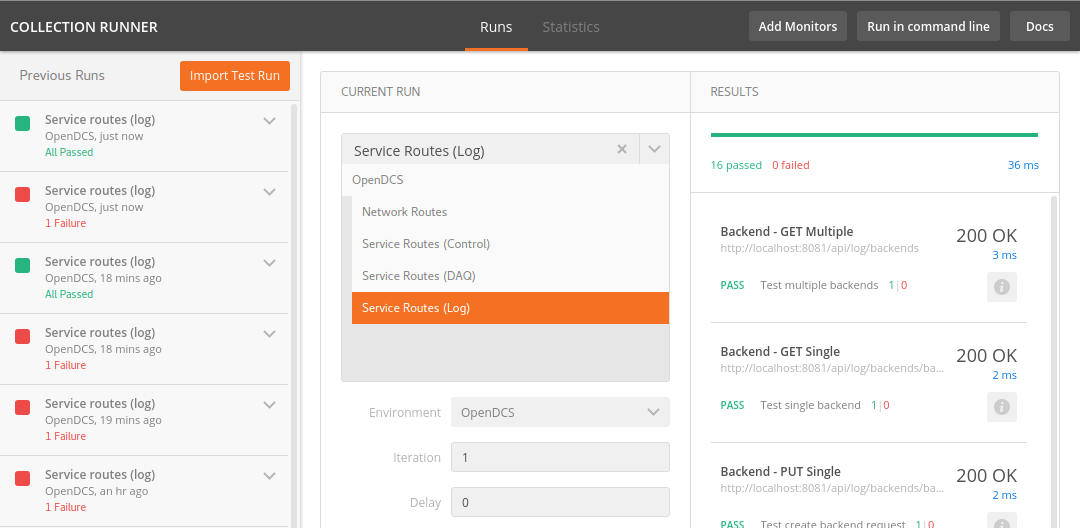
\includegraphics[width=\textwidth]{figures/testing/postman-log-suite-results}
          \caption{Test Suite Results for the Log Objects Tests}
          \label{fig:test-postman-log-suite}
        \end{figure}

    \subsubsection{Feedback Control Service Routes}\label{sec:test-rest-control}

      The API defined in Section~\ref{sec:rest-control} were those being tested
      in this context, and the configuration used to test against is below in
      Listing~\ref{lst:test-rest-control}.

      \lstinputlisting[language=Javascript,
                       caption={Configuration of Control Objects},
                       label={lst:test-rest-control}]
                      {testing/dcs-control.json}

      When the service is executed with this configuration the command
      \texttt{ss -antp4 | grep dcs-ctrl} shows the that the HTTP service as
      well as the ZeroMQ sockets have been correctly brought up and have a
      status of \texttt{LISTEN}, and the connecting pairs show \texttt{ESTAB},
      this output is given in Listing~\ref{lst:test-rest-control-ss}.

      \begin{lstlisting}[caption={Socket Status During Feedback Control Tests},
                         label={lst:test-rest-control-ss}]
        LISTEN 0 100 *:6001          *:*             users:(("dcs-ctrl",pid=12064,fd=15))
        LISTEN 0 10  *:8082           *:*            users:(("dcs-ctrl",pid=12064,fd=4))
        ESTAB  0 0   127.0.0.1:6001  127.0.0.1:35532 users:(("dcs-ctrl",pid=12064,fd=22))
        ESTAB  0 0   127.0.0.1:43448 127.0.0.1:5001  users:(("dcs-ctrl",pid=12064,fd=24))
        ESTAB  0 0   127.0.0.1:6001  127.0.0.1:53388 users:(("dcs-ctrl",pid=12064,fd=23))
      \end{lstlisting}

      \paragraph{Test Suite Run for this Scope}\mbox{}\\

      \begin{table}[H]
        \centering
        \begin{tabular}{p{3in} p{3in}}
          \toprule
          \emph{Request} & \emph{Description} \\ [0.5ex]
          \midrule
             GET /api/control/controllers       & Read multiple controllers \\
             GET /api/control/controllers/ctl1  &   Read single controller \\
             PUT /api/control/controllers/ctl1  &      Create a controller \\
            POST /api/control/controllers/ctl1  &      Update a controller \\
          DELETE /api/control/controllers/ctl1  &      Delete a controller \\
          \bottomrule
        \end{tabular}
        \caption{REST API Test Suite for Control Components}\label{tab:test-rest-control-suite}
      \end{table}

      \paragraph{Test Suite Results}\mbox{}\\

        All tests defined for the suite of control objects completed
        successfully, the results of the tests can be seen in
        Figure~\ref{fig:test-postman-control-suite}.

        \begin{figure}[H]
          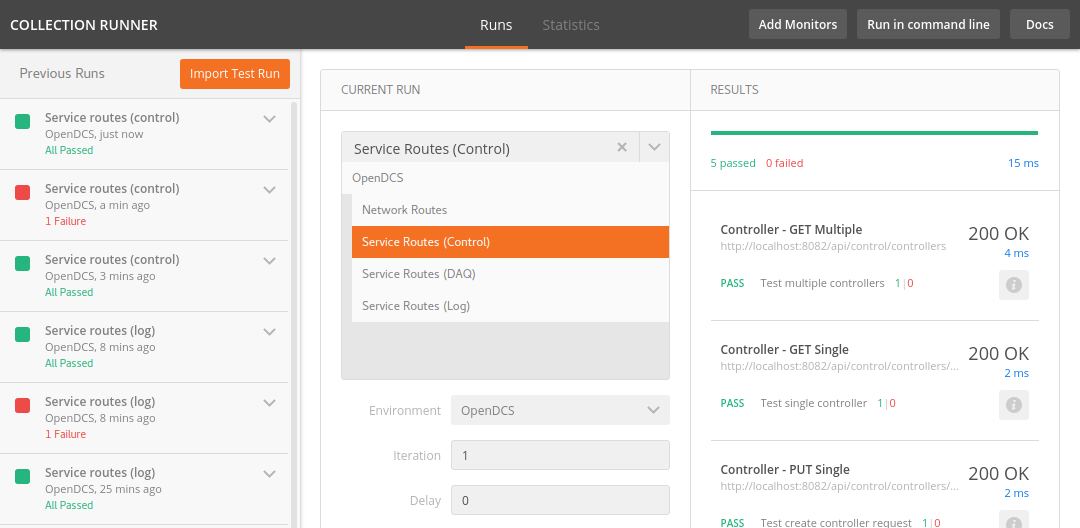
\includegraphics[width=\textwidth]{figures/testing/postman-control-suite-results}
          \caption{Test Suite Results for the Control Objects Tests}
          \label{fig:test-postman-control-suite}
        \end{figure}

  %\subsection{ZeroMQ Socket Channels}\label{sec:test-zeromq}

    %Commands used for testing \ldots

    %% Just here for reference for the time being
    %zmqc -r -c SUB 'tcp://127.0.0.1:5002' -o SUBSCRIBE=''
    %zmqc -r -c SUB 'tcp://127.0.0.1:5001' -o SUBSCRIBE='daq-test'
